\documentclass[11pt]{article}
\usepackage[margin=1in]{geometry}
\usepackage[utf8]{inputenc}
\usepackage[english]{babel}

\usepackage{pslatex}

\usepackage[pdftex]{graphicx}
\usepackage{siunitx}
\usepackage{caption}

\usepackage{booktabs,array}
\usepackage{tikz}
\usetikzlibrary{matrix,calc}
\usetikzlibrary{decorations.pathreplacing,angles,quotes}
\usetikzlibrary{bayesnet}
\usetikzlibrary{shapes.geometric,fit}

\newlength{\tikzheight}
\newlength{\tikzwidth}

\usepackage{amsfonts,amsmath,amssymb}
\usepackage{listings}
\usepackage{multicol}
\usepackage{multirow}
\usepackage{xcolor}
\usepackage{multicol}
\usepackage{algorithm}
\usepackage{algpseudocode}
\usepackage{adjustbox,lipsum}

\definecolor{c1}{RGB}{39,64,139}
\definecolor{c2}{RGB}{30,144,255}
\definecolor{c3}{RGB}{255,165,0}
\definecolor{c4}{RGB}{205,205,0}
\definecolor{c5}{RGB}{139,139,0}

\newcommand{\secref}[1]{\S\,\ref{#1}}
\newcommand{\appref}[1]{Appendix~\ref{#1}}
\newcommand{\figref}[1]{Fig.~\ref{#1}}
\newcommand{\tabref}[1]{Tab.~\ref{#1}}

\newcommand{\abs}[1]{\ensuremath\left|#1\right|}

\newcommand{\ie}{\emph{i.e.}}
\newcommand{\eg}{\emph{e.g.}}
\newcommand{\etc}{\emph{etc.}}

%
% The following macro is used to generate the header.
%
\newcommand{\lecture}[4]{
   \pagestyle{myheadings}
   \thispagestyle{plain}
   \noindent
   \begin{center}
   \framebox{
      \vbox{\vspace{1mm}
    \hbox to 6.58in {Technology and AI Learning Seminar (TAILS) \hfill Montana State University} 
    \hbox to 6.58in {Spring 2023 \hfill Dept. of Mathematics Sciences}
       \vspace{4mm}
       \hbox to 6.28in {\large\bf\hfill Lecture #1: #2  \hfill}
       \vspace{4mm}
       \hbox to 6.28in {\footnotesize Lecturer: #3 \hfill Scribe: #4}
      \vspace{1mm}}
   }
   \end{center}
   \markboth{Lecture #1: #2}{Lecture #1: #2}
   \vspace*{4mm}
}

\renewcommand{\vec}[1]{\ensuremath\bold{#1}}

\usepackage{biblatex}
\addbibresource{references.bib}
\usepackage{mathrsfs}

\begin{document}

%%%%%%%%%%%%%%%%%%%%%%%%%%%%%%%%%%%%%%%%%%%%%%%%%%%%%%%%%%%%%%%%%%%%%%%%%%%%%%%%%%%%%%%%%%%%%%%%%%%%%%%%%%%% FILL IN THE RIGHT INFO.
% \lecture{**LECTURE-NUMBER**}{**DATE**}{**LECTURER**}{**SCRIBE**}
\lecture{4}{Denoising and Filtering}{Dominique Zosso, 2023-02-24}{Derek Jollie}
\tableofcontents
\null\hrule

\section*{Preamble}
\begin{equation}
    u = u_0 + \eta
\end{equation}
We have an observed signal $u_o$, and we want to retrieve the signal of interest $u$ with minimized noise $\eta$.
We do this using the three approaches:
\begin{itemize}
    \item Convolution/Linear Filtering
    \item A variational approach including regularization
    \item A probabilistic framework.
\end{itemize}

\section{Convolution/Linear Filtering}
Since the signal is more locally correlated than the noise is not, we can try to recover $\Tilde{u}$ from $u_0$ by local averaging or convolution.  To do this, we set $g = \frac{1}{4}
\begin{bmatrix}
1 & 2 & 1
\end{bmatrix}$ (which is a centered "Gaussian"), and then $\Tilde{u}$ is given by
\begin{equation}
    \Tilde{u} = u_0 * (g * g)
\end{equation}
where $g*g = \frac{1}{16}
\begin{bmatrix}
    1 & 4 & 6 & 4 & 1
\end{bmatrix}$.

\subsection{Repeated Convolution}
We can visualize $g$ as $g = (x^{-\frac{1}{2}} + x^{\frac{1}{2}})^2$ since this is equivalent to $g = x^{-1} + 2 + x$.
So, $g * g = ((x^{-\frac{1}{2}} + x^{\frac{1}{2}})^2)^2$, and even
\begin{equation}
    g^n = (x^{-\frac{1}{2}} + x^{\frac{1}{2}})^{2n}.
\end{equation}
The binomial coefficients correspond to every other row in Pascal's triangle.
It follows that the binomial coefficients trend to a sampled Gaussian.
\begin{figure}
    \centering
    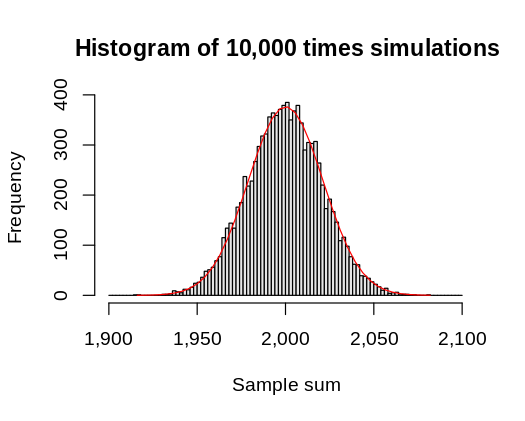
\includegraphics[scale=0.5]{figures/lecture04/central_limit_theorem.png}
    \caption{An illustration of the central limit theorem. \cite{wiki_1_2022}}
    \label{fig:Binomial Coefficients}
\end{figure}

\subsection{Spectral Side}
On the spectral side, the signal of interest becomes
\begin{equation}
    \Tilde{U} = U_0 \cdot G
\end{equation}
with 
\begin{equation}
    G(\nu) = \frac{1}{4}(e^{j2 \pi \nu \Delta} + 2 + e^{-j2 \pi \nu \Delta}) \\
        = \frac{1}{2} + \frac{1}{2}\cos (2 \pi \nu \Delta) 
\end{equation}
since $2\cos = e^j - e^{-j}$.
This acts as a low pass filter, leaving the lower frequencies untouched and damping the higher frequencies.

\begin{figure}
    \centering
    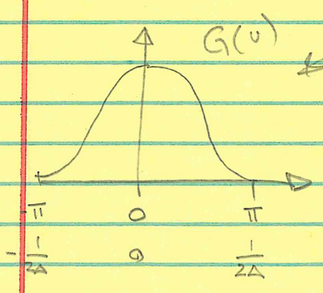
\includegraphics[scale=0.8]{figures/lecture04/Low_pass_filter.png}
    \caption{$G(\nu)$, the low pass filter.}
    \label{fig:Low Pass}
\end{figure}
\begin{figure}
    \centering
    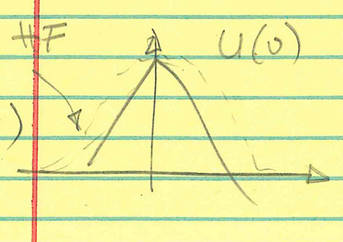
\includegraphics[scale=0.8]{figures/lecture04/U_from_filter.png}
    \caption{A visualization of applying the low pass filter on the signal.}
    \label{fig:Signal}
\end{figure}
\begin{figure}
    \centering
    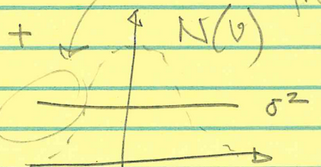
\includegraphics[scale=0.8]{figures/lecture04/White_noise.png}
    \caption{$\eta$, visualizing white noise.}
    \label{fig:White Noise}
\end{figure}
When the filter is applied as in \figref{fig:Signal}, the noise (as shown in \figref{fig:White Noise}) is damped around the edges.
For example, if we did this to a picture, the corners would be less distinct.

\section{Variational Approach}
Using
\begin{equation}\label{eq:Variational Approach}
    \Tilde{u} = \min_u \frac{1}{2}||u - u_0||_2^2
\end{equation}
yields the trivial solution $\Tilde{u} =u_0$, so some side side information is necessary.
This utilizes Tikhonov Regularization, so \eqref{eq:Variational Approach} can be written as
\begin{equation}\label{eq:Tikhonov}
    \Tilde{u} = \min_u \frac{1}{2}||u - u_0||_2^2 + R(u)
\end{equation}
where $R(u)$ is small for "good signals" which can be smooth and low energy.  In that case, they can be represented as $R(u) = \frac{\alpha}{2}||\nabla ||_2^2$.
Then, \eqref{eq:Tikhonov} can be written as
\begin{equation}
    \Tilde{u} = \min_u \frac{1}{2}||u - u_0||_2^2 + \frac{\alpha}{2}||\nabla ||_2^2.
\end{equation}
Then, the Euler--Lagrange equation is
\begin{equation}\label{eq:Euler--Lagrange}
    u - u_0 = \alpha \Delta u.
\end{equation}
The Fourier Transform diagonalizes the laplacian as $\Delta = X\Lambda X^H$ with $X = e^{-j2 \pi \nu t}$ being the eigenfunctions and $\Lambda = c\nu^2$ being the eigenvalues.
It can also be noted that $X$ is unitary.
Then, the Plancheral Theorem results in $||f||_2^2 = ||F||_2^2$, but it can be noted that the same result utilizing inner products can be found using Parserval's Theorem.
Therefore, on the spectral side, \eqref{eq:Euler--Lagrange} becomes
\begin{equation}
    \Tilde{U} = \min_U \frac{1}{2}||U-U_0||_2^2 + \frac{\alpha}{2}(2\pi \nu)^2 ||U||_2^2
\end{equation}
\subsection{Low-Pass Filter}
\begin{equation}
    \begin{split}
        \mathscr{F}(\frac{d}{dt}f) &= \int \frac{d}{dt}f e^{-j2 \pi \nu t}dt\\
        &= - \int f \frac{d}{dt} e^{-j2 \pi \nu t}dt\\
        &= -j2 \pi \nu \int fe^{-j2 \pi \nu t}dt\\
        &= -j2 \pi \nu \mathscr{F}(\nu)
    \end{split}
\end{equation}
Then it follows that 
\begin{equation}
    \begin{split}
        U - U_0 = \frac{\alpha}{2}(2\pi \nu)^2 U\\
        \Tilde{U} = \frac{U_0}{1 + \alpha(2\pi \nu)^2}.
    \end{split}
\end{equation}
Which is the low-pass filter.

\section{Probabilistic Approach}
Now, we are going to assume
\begin{equation}
        u_0 = u + \eta 
\end{equation}
with $\eta \sim N(0, \sigma^2)$.
So $u_0 \sim (u,\sigma^2)$, and if we have observed data $u_0$, what is the most likely $u$ that produced that data.
We can see
\begin{equation}
    P(u_0|u) = N(u_0| u, \sigma^2),
\end{equation}
and using the maximum likelihood estimate, it should follow that we get $u = u_0$ which again is too trivial.
There needs to be some priors, and then we can try using Bayes.
The prior used is $P(\nabla u): \nabla u \sim N(0, I)$.
Now, $\max_u P(u| u_0) \propto P(u_0|u) \cdot P(u)$, and we can take the negative log and minimize it instead which will lead to
\begin{equation}
    \min_u \frac{1}{2\sigma^2}||u - u_0||^2 + \frac{1}{2}||\nabla u||^2
\end{equation}
\end{document}